\documentclass{beamer}

% Theme choice
\usetheme{Madrid}

% Optional packages
\usepackage{graphicx} % For including images
\usepackage{amsmath}  % For math symbols and formulas
\usepackage{hyperref} % For hyperlinks
\usepackage{listings}
\usepackage{xcolor}
\usepackage{tikz}
\usepackage[T1]{fontenc}

\lstdefinestyle{CStyle}{
  language=C,                    % Set the language to C
  basicstyle=\ttfamily\footnotesize\linespread{0.9}\tiny, % Set font style and size
  keywordstyle=\color{blue},      % Color of keywords
  commentstyle=\color{gray},      % Color of comments
  stringstyle=\color{red},        % Color of strings
  showstringspaces=false,         % Do not mark spaces in strings
  breaklines=true,                % Enable line breaks at appropriate places
  breakatwhitespace=false,        % Break lines at any character, not just whitespace
  numbers=left,                   % Show line numbers on the left
  numberstyle=\tiny\color{gray},  % Style for line numbers
  tabsize=4,                      % Set tab width
  keepspaces=true,                % Keep indentation spaces
  frame=single,                   % Add a border around the code
  aboveskip=0pt,                  % Reduce space above the code block
  belowskip=0pt,                   % Reduce space below the code block
  xleftmargin=7.5pt,                      % Add left padding (approx. 2.8mm or 10px)
  xrightmargin=15pt,                      % Add left padding (approx. 2.8mm or 10px)
}

% Title, author, date, and institute (optional)
\title[Parallel Programming. Repository structure]{Parallel Programming course. Repository structure}
\author{Obolenskiy Arseniy, Nesterov Alexander}
\institute{Nizhny Novgorod State University}

\date{\today} % or \date{Month Day, Year}

% Redefine the footline to display both the short title and the university name
\setbeamertemplate{footline}{
  \leavevmode%
  \hbox{%
    \begin{beamercolorbox}[wd=.45\paperwidth,ht=2.5ex,dp=1ex,leftskip=1em,center]{author in head/foot}%
        \usebeamerfont{author in head/foot}\insertshortinstitute % Displays the university name
    \end{beamercolorbox}%
    \begin{beamercolorbox}[wd=.45\paperwidth,ht=2.5ex,dp=1ex,leftskip=1em,center]{author in head/foot}%
      \usebeamerfont{author in head/foot}\insertshorttitle % Displays the short title
    \end{beamercolorbox}%
    \begin{beamercolorbox}[wd=.1\paperwidth,ht=2.5ex,dp=1ex,rightskip=1em,center]{author in head/foot}%
      \usebeamerfont{author in head/foot}\insertframenumber{} / \inserttotalframenumber
    \end{beamercolorbox}}%
  \vskip0pt%
}

\begin{document}

\begin{frame}
    \titlepage
\end{frame}

\begin{frame}{Contents}
    \tableofcontents
\end{frame}

\section{The introduction to the repository}

\begin{frame}[fragile]{Parallel programming technologies}
  \begin{itemize}
    \item \textbf{MPI}
    \item OpenMP
    \item TBB
    \item std::thread
  \end{itemize}
\end{frame}

\begin{frame}[fragile]{Step-by-step guide to build the project}
  \begin{itemize}
    \item Download all submodules
    \item Set up your environment
    \item Build the project with CMake
  \end{itemize}
\end{frame}

\begin{frame}[fragile]{Download all submodules \& Set up your environment}

  \lstset{style=CStyle, caption=Git submodules}
  \begin{lstlisting}
    git submodule update --init --recursive
  \end{lstlisting}

    \lstset{style=CStyle, caption=Download MPI}
  \begin{lstlisting}
    // Windows
    msmpisdk.msi & msmpisetup.exe
    // Linux (gcc and clang)
    sudo apt install -y mpich openmpi-bin libopenmpi-dev
    // MacOS (apple clang)
    brew install open-mpi
  \end{lstlisting}

\end{frame}

\begin{frame}[fragile]{Build the project with help CMake}

  \lstset{style=CStyle, caption=Configure the build}
  \begin{lstlisting}
    cmake -S <source code/path to CMakeLists.txt> \
          -B <build directory> \
          -D USE_SEQ=ON \
          -D USE_MPI=ON \ 
          -D USE_FUNC_TESTS=ON \
          -D USE_PERF_TESTS=ON \
          -D CMAKE_BUILD_TYPE=Release ..
  \end{lstlisting}

  \lstset{style=CStyle, caption=Build the project}
  \begin{lstlisting}
    cmake --build <build directory> \
          --config Release \
          --parallel
  \end{lstlisting}

\end{frame}

\section{How to submit your work}

\begin{frame}[fragile]{Directories}
  \begin{table}[h!]
    \resizebox{8cm}{!} {
      \begin{tabular}{| p{4.2 cm} | p{4.2 cm} |}
      \hline
      \textbf{Directory} & \textbf{What is it?} \\
      \hline
      \textbf{.github/workflows} & CI \\
      \hline
      \textbf{1stsamples} & Simple examples \\
      \hline
      \textbf{3rdparty} & Auxiliary libraries \\
      \hline
      \textbf{cmake} & CMake scripts \\
      \hline
      \textbf{modules} & API source code \\
      \hline
      \textbf{scripts} & Auxiliary scripts \\
      \hline
      \textbf{tasks} & Students tasks \\
      \hline
    \end{tabular}
    }
    \caption{Root directories}
  \end{table}

  \begin{table}[h!]
    \resizebox{8cm}{!} {
    \begin{tabular}{| p{4.2 cm} | p{4.2 cm} |}
      \hline
      \textbf{Directory} & \textbf{What is it?} \\
      \hline
      \textbf{mpi} & MPI \\
      \hline
      \textbf{omp} & OpenMP \\
      \hline
      \textbf{seq} & Sequential \\
      \hline
      \textbf{stl} & std:thread \\
      \hline
      \textbf{tbb} & Threading Building Blocks \\
      \hline
    \end{tabular}
    }
    \caption{Tasks directories}
  \end{table}

\end{frame}

\begin{frame}[fragile]{Directories}
  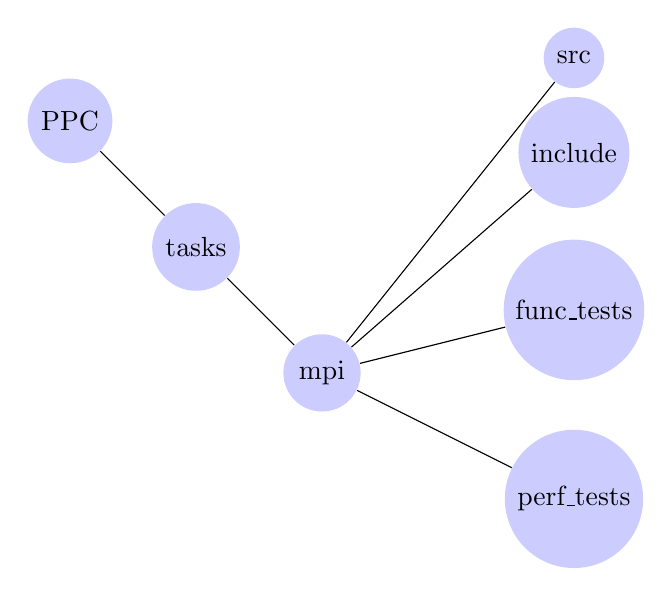
\begin{tikzpicture}
  [scale=.8,auto=left,every node/.style={circle,fill=blue!20}]
  \node (n1) at (1,10) {PPC};
  \node (n2) at (3,8)  {tasks};
  \node (n3) at (5,6)  {mpi};
  \node (n4) at (9,11)  {src};
  \node (n5) at (9,9.5) {include};
  \node (n6) at (9,7) {func\_tests};
  \node (n7) at (9,4) {perf\_tests};

  \foreach \from/\to in {n1/n2,n2/n3,n3/n4,n3/n5,n3/n6,n3/n7}
    \draw (\from) -- (\to);

\end{tikzpicture}
\end{frame}

\begin{frame}{References}
  \begin{itemize}
    \item PPC Repository \href{https://github.com/learning-process/parallel\_programming\_course}{https://github.com/learning-process/parallel\_programming\_course}
  \end{itemize}
\end{frame}

\end{document}
